%Correct the file name.
%X: book number
%Y: part number
%ZZZ: page number in three digits. So page 3 would be 003.

\documentclass[11pt]{amsbook}

\usepackage{../HBSuerDemir}	% ------------------------


\begin{document}

% ++++++++++++++++++++++++++++++++++++++
\hPage{b2p2/429}
% ++++++++++++++++++++++++++++++++++++++

\section*{2. Mass, moments, center of grevity. moments of inertia}

By the usual notations

$m=\iiint \limits_{\mathbb{R}} \delta(x,y,z)dV$

$M_{xy} = \iiint \limits_{\mathbb{R}} z \delta dV$, $M_{xz} = \iiint \limits_{\mathbb{R}} y \delta dV$, $M_{yz} = \iiint \limits_{\mathbb{R}} x \delta dV$

$G(M_{yz}/m, M_{xz}/m, M_{xy}/m)$
\newline
$I_{ox}=\iiint \limits_{\mathbb{R}} (y^2+z^2) \delta dV$ , $I_{oy}=\iiint \limits_{\mathbb{R}} (x^2+z^2) \delta dV$ , $I_{oz}=\iiint \limits_{\mathbb{R}} (x^2+y^2) \delta dV$
and in general
\newline
$M_{\pi} = \iiint \limits_{\mathbb{R}} d(P,\pi) \delta dV$ , $M_{\ell} = \iiint \limits_{\mathbb{R}} d(P,\ell) \delta dV$ , $M_{A} = \iiint \limits_{\mathbb{R}} d(P,A) \delta dV$
\newline
$I_{\pi} = \iiint \limits_{\mathbb{R}} d^2(P,\pi) \delta dV$ , $I_{\ell} = \iiint \limits_{\mathbb{R}} d^2(P,\ell) \delta dV$ , $I_{A} = \iiint \limits_{\mathbb{R}} d^2(P,A) \delta dV$

Example. Find the centroid ($\delta$ is constant) of the solid bounded by $x^2+y^2+z^2=a^2$, in the first octant.

Solution. From symmetry we have $\overline{x} = \overline{y} = \overline{z}$.

\begin{tabular}{lll}
	\multicolumn{3}{l}{$m = \delta V = \frac{6}{\delta} \pi a^3$}  \\
	$m\overline{z}$ & $=$ & $ M_{xy} = \int_{0}^{\pi/2}\int_{0}^{\pi/2}\int_{0}^{a} \rho \cos\varphi \rho^2 \sin\varphi d\rho d\varphi d\theta$ \\
	& $=$ & $ \frac{\delta}{2} \int_{0}^{\pi/2}\int_{0}^{\pi/2}\int_{0}^{a} \rho^3 d\rho \sin{2\varphi}d\varphi d\theta$ \\
	& $=$ & $ \frac{\pi}{8} a^4 \int_{0}^{\pi/2}\int_{0}^{\pi/2} \sin{2\varphi}d\varphi d\theta$ \\
	& $=$ & $ \frac{\delta}{8} a^4 \frac{\pi}{2} = \frac{\delta}{16} \pi a^4$ \\
	& & $\overline{x} = \overline{y} = \overline{z} = \frac{\delta}{16} \pi a^4 / (\frac{\delta}{6} \pi a^3) = \frac{3}{8}a$
\end{tabular}

% =======================================================
\end{document}  

%==== templates ====

%==== environments ====

%\begin{figure}[htb]
%	\centering
%	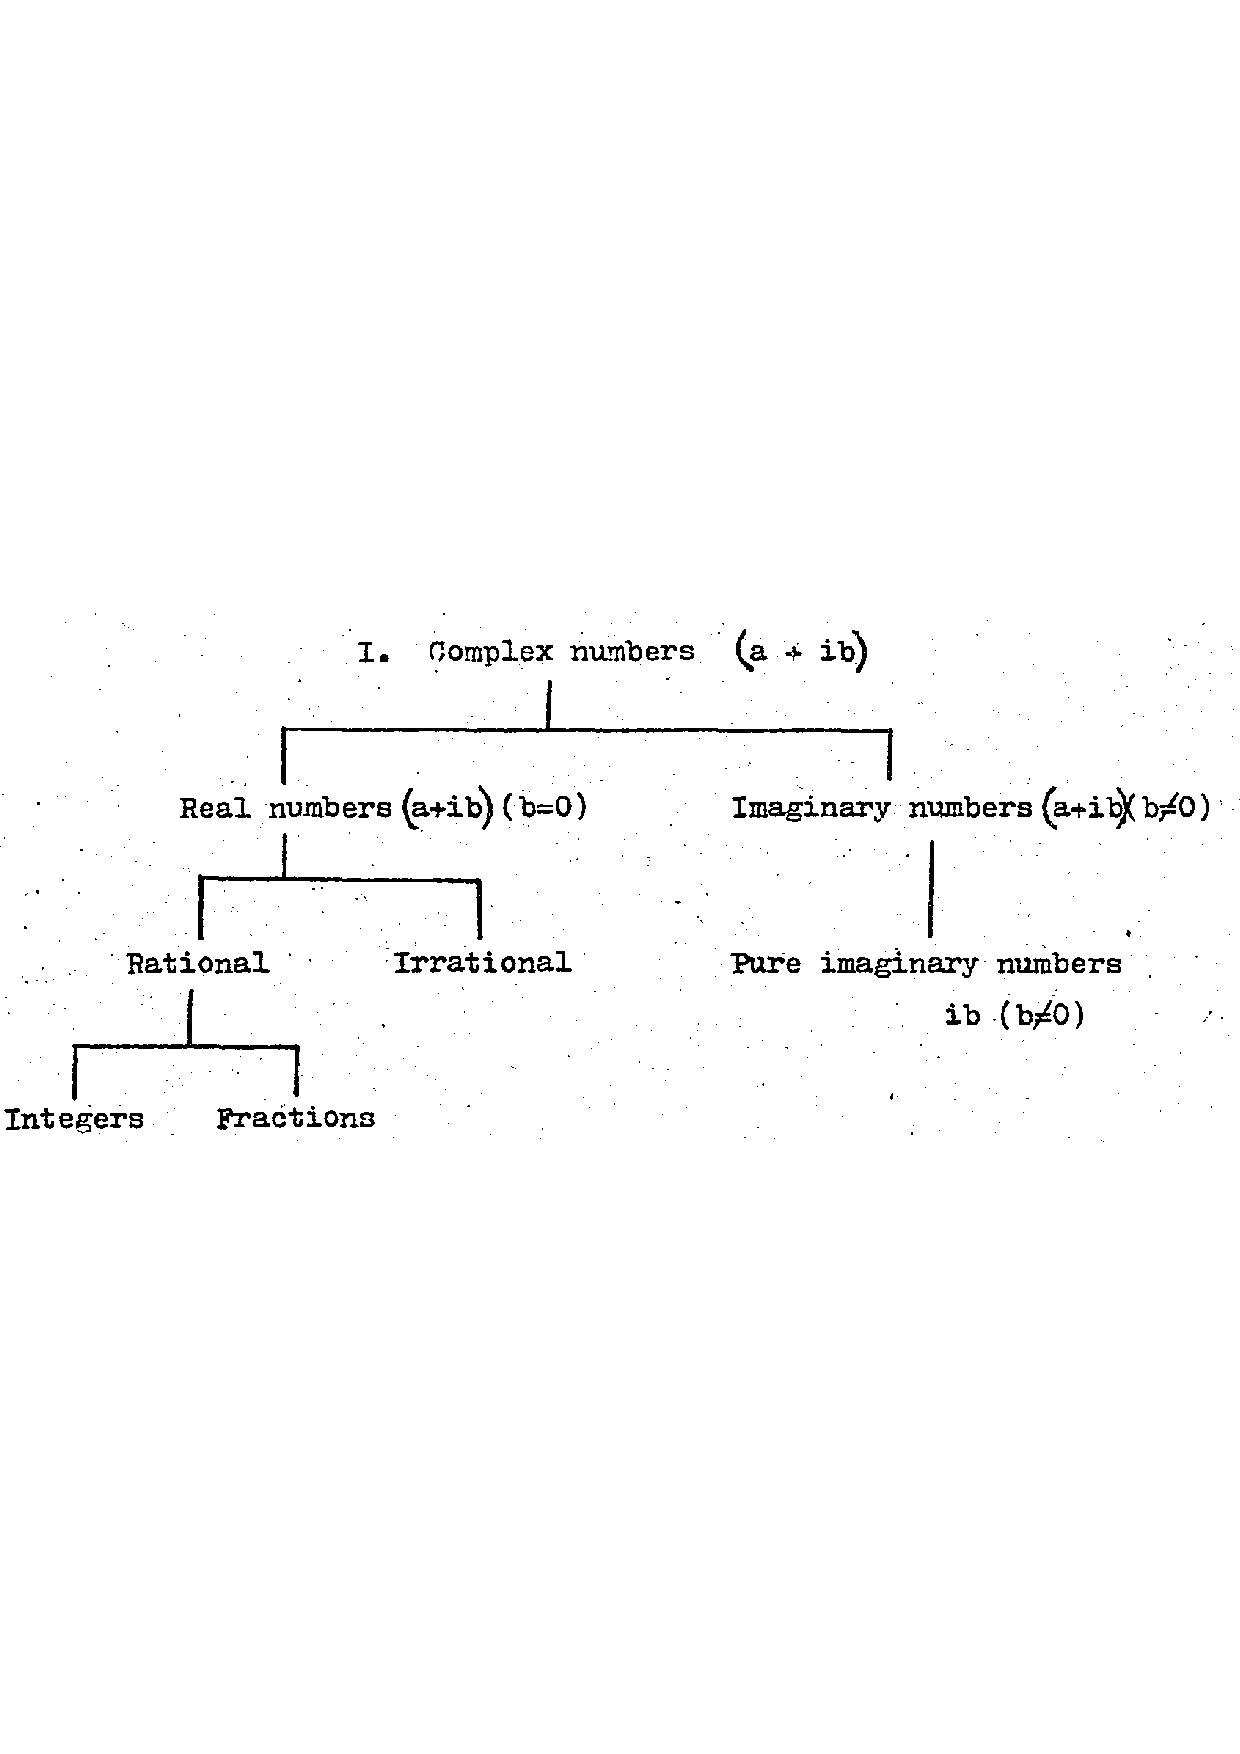
\includegraphics[width=0.9\textwidth]{images/SD-1-1p15A}
%	\caption{Classification of complex numbers}
%	\label{fig:classificationOfComplexNumbersA}
%\end{figure}

%\begin{center}
%\begin{tabular}{cc}
%\end{tabular}
%\end{center}

%\begin{exmp}
%\begin{hSolution}
%\end{hSolution}
%\end{exmp}

%\begin{hEnumerateAlpha}
%\end{hEnumerateAlpha}

%\begin{hEnumerateRoman}
%\end{hEnumerateRoman}

%$
%\begin{bmatrix}
%\end{bmatrix}
%$

%\frac{aaaa}{bbb}
%\frac{a_{n}}{b_{n}}
%\left( aaaa \right)
%\Longrightarrow

%\begin{multicols}{2}
%	bb
%\columnbreak
%	aa
%\end{multicols}
